\documentclass[11pt,twoside,titlepage]{article}
\usepackage[tc]{titlepic}
\usepackage{times}
\usepackage{float}
\usepackage{amssymb}
\usepackage{amsmath}
\usepackage{amsthm}
\usepackage{needspace}
\usepackage{url}
\usepackage{hyperref}
%\usepackage{mathptm}
\usepackage{fancyhdr}
\usepackage{wrapfig}
\ifx\pdfoutput\undefined
% we are running LaTeX, not pdflatex
\usepackage{epsfig,color}
\else
% we are running pdflatex, so convert .eps files to .pdf
\usepackage[pdftex]{epsfig,color}
\usepackage{epstopdf}
\usepackage{pdfsync}
\fi
\usepackage{ifthen,version}
\usepackage{listings}
%\usepackage{temporal}
%\usepackage{algorithmic}
\newboolean{print-solutions}

% Start of configuration section
% Comment out the following line to exclude the printing of solutions.
%\setboolean{print-solutions}{true}
\newcommand{\labnumber}{1}
\newcommand{\labname}{Digital Logic Gates}
\newcommand{\coursenumber}{MobaXterm and SSH How-To Document}
\newcommand{\coursename}{Introduction to Digital Design}
% End of configuration section

% Conditional definitions
\newcommand{\dateorsol}{\LARGE \ifthenelse{\boolean{print-solutions}}%
  {Solutions}{Due \duedate}}
\newcommand{\headertxt}{\sl \ifthenelse{\boolean{print-solutions}}%
  {Solutions to}{} Laboratory Exercise \#\labnumber}
\newcommand{\points}[1]{\ifthenelse{\boolean{print-solutions}}%
  {}{[#1 points.]}}
\ifthenelse{\boolean{print-solutions}}{\includeversion{prnt-solns}}%
{\excludeversion{prnt-solns}}

\textwidth=7.25in
\evensidemargin=-0.35in
\oddsidemargin=-0.35in

\newcommand{\ite}{\operatorname{ite}}
\newcommand{\itec}{\operatorname{ite\_constant}}

{\theoremstyle{definition} \newtheorem{definition}{Definition}}
\newtheorem{theorem}{Theorem}
\newtheorem{lemma}{Lemma}
\newtheorem{corollary}{Corollary}
\newtheorem{proposition}{Proposition}
{\theoremstyle{remark}
  \newtheorem{example}{Example}
  \newtheorem{problem}{Problem}
  \newtheorem{note}{Note}}
% Fortunately, proofs can be nested.
\newenvironment{solution}{\begin{proof}[Solution]}{\end{proof}}


\newcommand{\ta}{Created By: Kyler Scott and Prof. Sunil P. Khatri\\July 2020}
\title{ \huge Department of Electrical and Computer Engineering\\ \huge Texas A\&M University \\}
\author{ \huge MobaXterm and SSH:\\ \\ \huge How-To Document \\ \\ \\ \ta}

\titlepic{
\includegraphics[width=0.5\textwidth]{logo}}

\date{}
\pagestyle{fancy}
\lhead[\rm\thepage]{}
\rhead[]{\rm\thepage}
\lfoot[]{\coursenumber}
%\cfoot{\instructor}
\rfoot[\coursenumber]{}

\begin{document}
\bibliographystyle{alpha}
\maketitle

\noindent
\textbf{Note:} This guide is intended for students running the Windows OS. If you are a Mac user, you must first set up an instance of the Windows OS on your Mac. For this, refer to the "Bootcamp How-To Document" for instructions on how to use Bootcamp to run Windows OS on your Mac machine. After you are running the Windows OS, you can follow the steps described in this document to use MobaXterm.\\

\section{Introduction}
Students in ECEN 449 will need to connect to the on-campus Linux machines using an SSH (Secure Shell) connection. MobaXterm is one software program that makes this task possible, by providing a graphical user interface (GUI) that allows you to view the shell on the on-campus Linux machine, see the filesystem structure, and save commonly-used connections. This guide will describe the basics of MobaXterm for initiating and using an SSH connection, as well as creating a serial port connection.\\

\section{Installing MobaXterm}

\noindent
Visit the \href{https://mobaxterm.mobatek.net/download.html}{MobaXterm downloads page} and under the Home Edition, click "Download now". Click "MobaXterm Home Edition (Installer edition)" button to download the installer .zip file. It does not matter where you save this file.\\

\noindent
Navigate to the .zip file you downloaded and extract the files by right clicking the .zip file and selecting "Extract All". Once this is done, navigate to the extracted files. Right click on the .msi file and click "Install". A window should open up which looks like Figure~\ref{install}.\\

\begin{figure}[!h]
	\centering 
	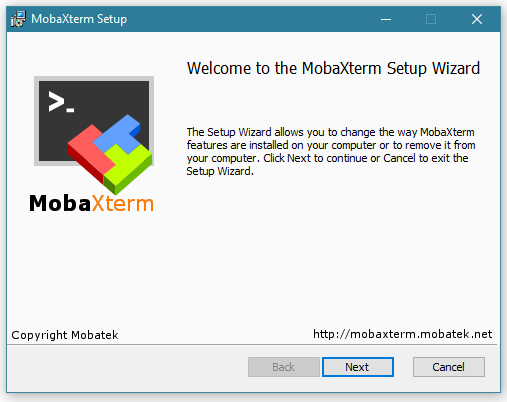
\includegraphics[ width=.4\textwidth]{install}
	\caption{MobaXterm Installer Welcome Page}
	\label{install}
\end{figure}

\noindent
Click "Next", accept the license agreement, and click "Next" again. Select a location to install MobaXterm, click "Next" and then "Install".\\




\section{SSH Connection (ECEN 449/749 Labs 4-7)}

\noindent Open MobaXterm. You should see a window similar to Figure~\ref{xterm_start}. To create an SSH connection, click on the "Session" button on the top left corner of the screen. Select "SSH", and enter the name of the remote host you wish to connect to. For the ECEN 449/749 labs, this host will be "olympus.ece.tamu.edu". Select "Specify username" and in the box next to it, enter the username of your ECE account. Leave the port as the default port (22). Your window should look like Figure~\ref{xterm_ssh}.\\

\noindent
\textbf{Note:} Your ECE account username and password are likely identical to your NetID and password. Contact the TAMU Helpdesk if you are unable to access your ECE account, or if you have not yet set one up.

\begin{figure}[!h]
	\centering 
	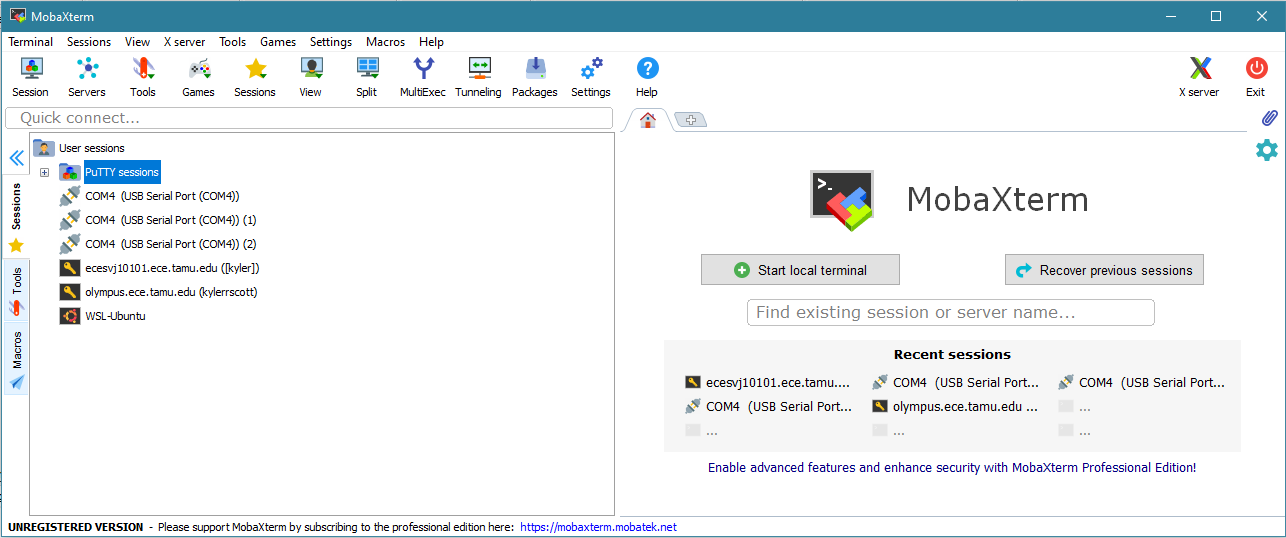
\includegraphics[ width=.8\textwidth]{xterm_start}
	\caption{MobaXterm Start Page}
	\label{xterm_start}
\end{figure}

\begin{figure}[!h]
	\centering 
	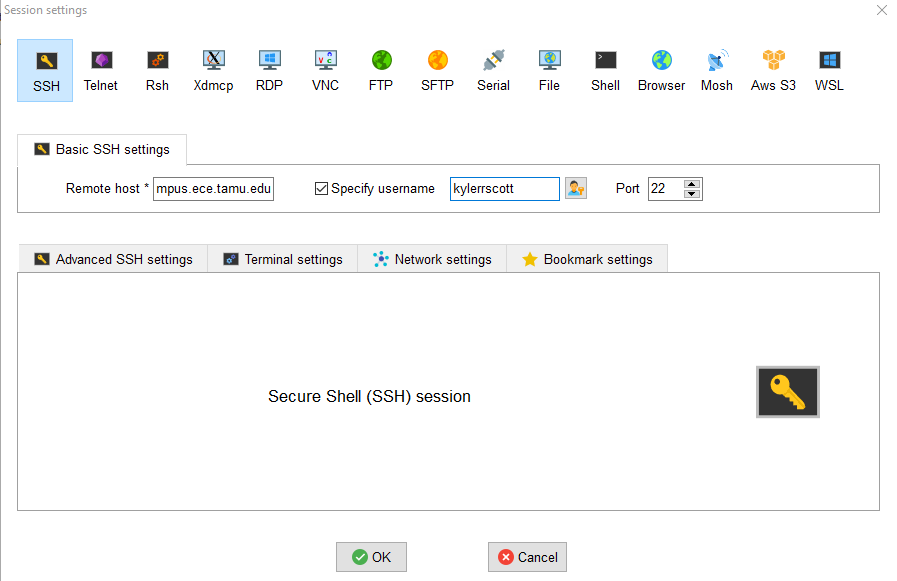
\includegraphics[ width=.6\textwidth]{xterm_ssh}
	\caption{MobaXterm: Open SSH Connection}
	\label{xterm_ssh}
\end{figure}

\noindent
Click "OK" to open the connection. A shell should appear and ask you for your password. Once you have entered your password and pressed 'enter', you will be properly connected and ready to use the shell.\


\section{Serial Port Connection (ECEN 449/749 Labs 4-7)}

\noindent
In some ECEN 449 labs, we will need to display messages coming from the Zybo board and into our computer's USB port. In order to see these messages, we will need to open a serial port connection.\\

\noindent
To create a serial connection, open MobaXterm. Click on the "Session" button on the top left corner of the screen and select "Serial". To connect to the Zybo board, under Serial port type "COM4" and under Speed type "115200". Your screen should look like Figure~\ref{xterm_com4}.\\


\begin{figure}[!h]
	\centering 
	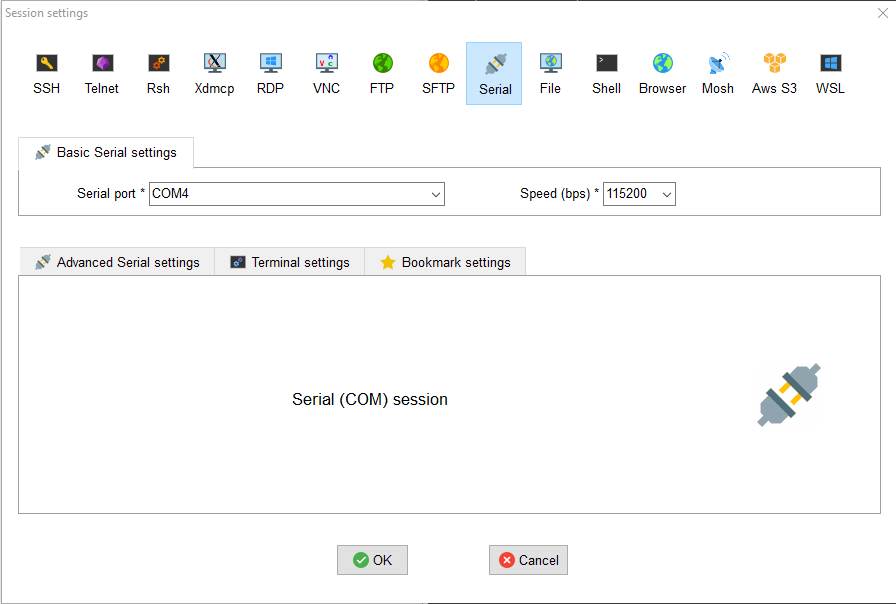
\includegraphics[ width=.6\textwidth]{xterm_com4}
	\caption{MobaXterm: Open Serial Connection to COM4}
	\label{xterm_com4}
\end{figure}

\noindent
Press "OK" to open the serial connection. Note that if your Zybo board is not connected to your computer and turned on, this connection will not be able to open. Once you open the connection, if you unplug or power off the Zybo board, you will have to reopen the connection.\\

\section{Downloading and Uploading Files (ECEN 449/749 Labs 4-7)}

\noindent
In many of the ECEN 449 labs, you will be required to download files from the ECE server to your local machine. Fortunately, this is easy with MobaXterm. Once you have opened an SSH connection, you will see a GUI displaying the remote filesystem on the left side of your screen, as shown in Figure~\ref{filesystem}.\\



\begin{figure}[!h]
	\centering 
	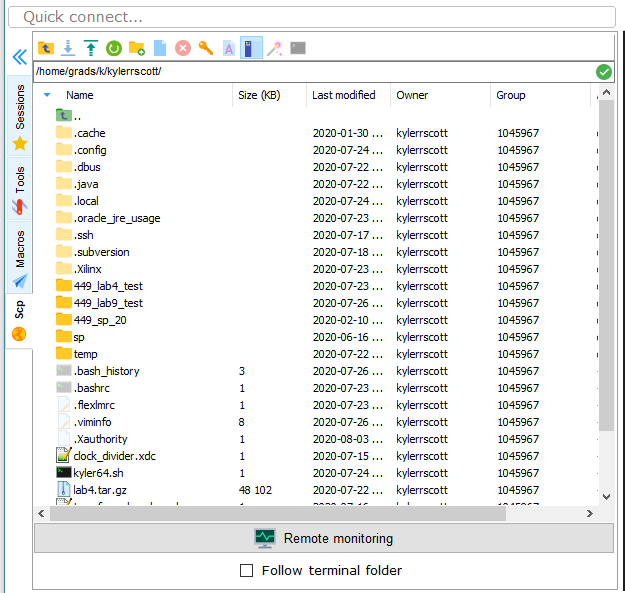
\includegraphics[ width=.5\textwidth]{filesystem}
	\caption{Remote Filesystem GUI (left side of screen after opening SSH connection)}
	\label{filesystem}
\end{figure}

\noindent
You can use this GUI to navigate through directories. To download files, navigate to the directory they are in, select them, right click and press "Download". You will then select a destination directory (on your local PC) and click "OK". The download will then begin.\\


\end{document}

